\newpage
\appendix
\renewcommand{\thechapter}{\Asbuk{chapter}}
\chapter{Описание приложения trowth.exe} 
\section{Отличительные особенности} \label{app1start}

Программа представляет собой отдельное кроссплатформенное приложение с графическим интерфейсом, написанное на языке высокго уровня JavaSE 7u75. Для построения графического интерфейса был использован фреймворк JavaFX.	

Отличительными особенностями приложения являются:
\begin{itemize}
\item{Математический пакет собственной разработки, а так же модуль наглядного отображения и ввода  математических формул. Модуль полностью построен на векторной графике, что позволяет редактору адаптироваться под любые разрешения экрана, описанная идея ранее нигде не использовалась и полностью принадлежит автору.}
\item{В данном продукте реализована идея живого приложения, по возможности автор освобождает пользователя от нажатия на лишние кнопки. Как только пользователь вносит малейшее изменение в параметры, графики, изменяет формулы, незамедлительно происходят все необходимые перерасчеты и перепостроения. Например, в основном разделе моделирования не используется не единой кнопки, а благодаря многопоточной оптимизации внутренних расчетов производительность интерфейса практически не снижается.}
\item{Векторный движок собственной разработки, благодаря нему программный продукт выглядит одинаково хорошо как на большом мониторе, так и на экране мобильного телефона. Кроме того реализована возможность программного сглаживания готового изображения, что позволяет рисовать дробную часть пикселя и в конечном итоге позволяет получить наилучшее отображение графиков и текста.}
\end{itemize}

Все изображения, используемые в приложении защищены авторским правом, алгоритмы и методы, используемые в приложении являются интеллектуальной собственностью автора. Стабилизация движения трехколесного робота . Патент РФ на программу для ЭВМ №201561534.  Москва, Роспатент, заявка № 2015612544. Дата поступления 25.03.2015.  Дата государственной регистрации в Реестре программ для ЭВМ 15.05.2015. 

Приложение предназначено для моделирования управляемого движения трехколесного робота, анализа качества управления, скорости выхода робота на желаемую траекторию движения, результаты математического моделирования которого используются в параграфе 3.3 главы 3 настоящей диссертации.

Моделирование начинается с запуска приложения trowth.exe для Windows и trowh.jar - для Linux, в основном меню рис.\eqref{ris:window} программы пользователю предоставляется возможность ознакомиться с теоретической частью, лежащей в основе математического моделирования управляемого движения колесного робота, ознакомиться с информацией об авторах проекта или перейти к демонстрации работы заложенного закона управления. 

\begin{figure}[h]
\center{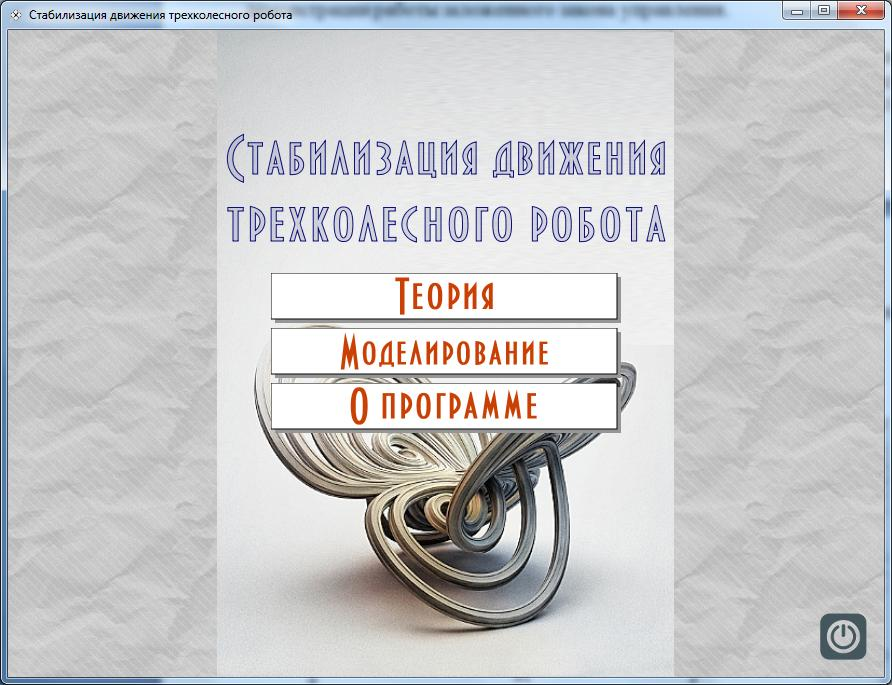
\includegraphics[width=1\linewidth]{window}}
\caption{Основной экран программы}
\label{ris:window}
\end{figure}

\par
\textbf{Теоретический раздел}

В теоретическую часть входит схематическое изображения управляемого объекта, система дифференциальных уравнений, описывающая движение робота и описание характеристик, использующихся в построении управления рис.\eqref{ris:theory}. 
Подробные теоретические выкладки содержатся в главе 3 настоящей  диссертации.
\nopagebreak[4]
\begin{figure}[h]
\center{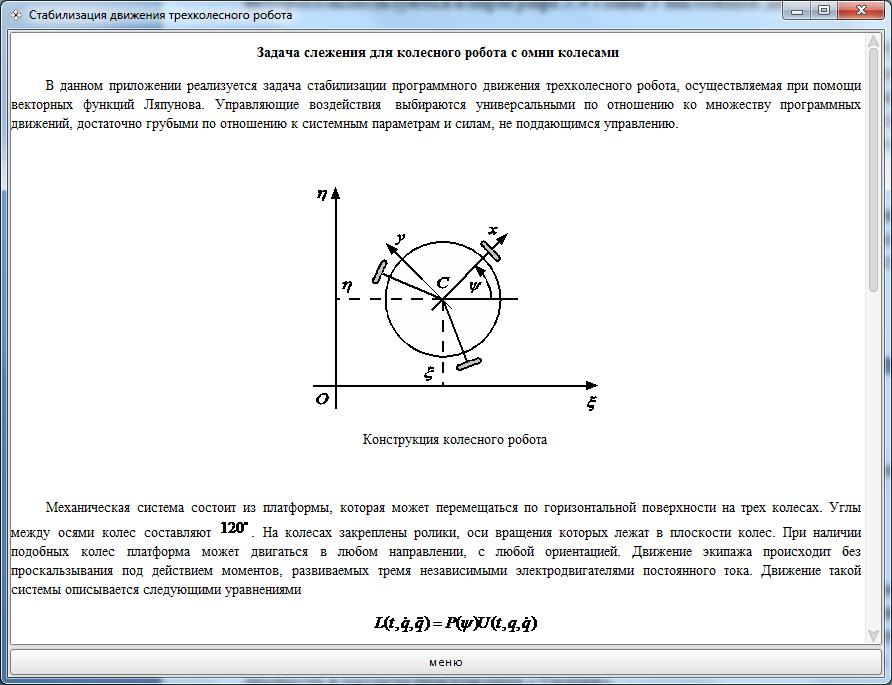
\includegraphics[width=1\linewidth]{theory}}
\caption{Внешний вид теоретического раздела}
\label{ris:theory}
\end{figure} 

\par
\textbf{Раздел моделирование}

При переходе непосредственно к математическому моделированию пользователю предлагается задать параметры системы, параметры управления, а так же начальные точки положения робота, либо согласиться с предложенными рис.\eqref{ris:params}. О значении каждого из параметров пользователь может прочесть в разделе приложения «Теория».

\begin{figure}[h]
\center{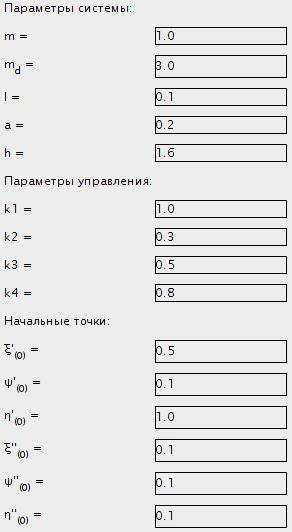
\includegraphics[width=0.5\linewidth]{params}}
\caption{Параметры для расчетов}
\label{ris:params}
\end{figure} 

Следующим этапом работы с программой является задание движения робота одним из следующих способов рис.\eqref{ris:modeling}:
\begin{enumerate}
\item{Аналитический ввод функций, описывающих движение робота;}
\item{Задание траектории движения графически;}
\item{Загрузить файлы с массивами данных.}
\end{enumerate}

\begin{figure}[h]
\center{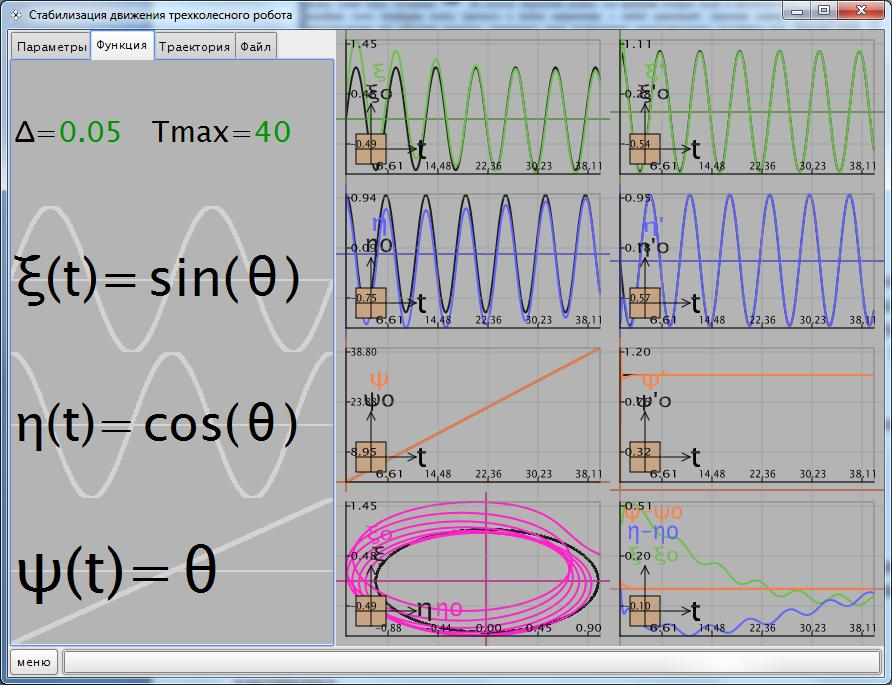
\includegraphics[width=1\linewidth]{modeling}}
\caption{Внешний вид раздела моделирование}
\label{ris:modeling}
\end{figure}

В случае возникновения ошибки на одном из этапов ввода данных, пользователь незамедлительно увидит предупреждение о некорректном вводе и возможных методах исправления ошибки.
\par
\textbf{Задание закона движения робота аналитически}

Ввод формул данным методом задействует достаточно мощный математический пакет самостоятельно разработанный автором. 

Использование векторной графики позволило сделать ввод формулы интерактивным, формула во время ввода автоматически занимает все доступное для нее место, в правой части стоит приглашение к вводу в виде знака "[?]". При клике мыши на этот значок выпадает список с вариантами возможных операций. Процесс создания формулы ведется путем собирания формулы из отдельных функциональных блоков. После ввода формулы происходит её компиляция в оперативную память и при каждом следующем обращении процессор практически не участвует в вычислении, за счет этого достигается высокая скорость производительности пакета. 
Стоит отметить, что тестирование скорости обработки формул математическим пакетом, выявило его преимущество перед такими известными инструментами, как MathCad 14 и Maple 12. Несомненно, преимущество в скорости обусловлено относительно скромным набором функций, входящих в арсенал разработанного продукта, однако, библиотека формул является более чем достаточной для проведения моделирования и может быть расширена при необходимости.

Для более подробного ознакомления с реализацией математического пакета см. Приложение 2-2.4.

На первом этапе пользователю предлагается ввести функции   $\xi = \xi_0(t), \eta = \eta_0(t), \psi = \psi_0(t)$, описывающие движение робота, а так же шаг дискретизации $\delta$  и время моделирования  $T_{max}$ рис.\eqref{ris:formul}. По мере введения каждой функции под ней рисуется миниатюра графика, что позволяет ориентироваться и подбирать коэффициенты в сложных формулах. По окончанию ввода последней формулы незамедлительно происходит моделирование управляемого движения робота.

\begin{figure}[h]
\center{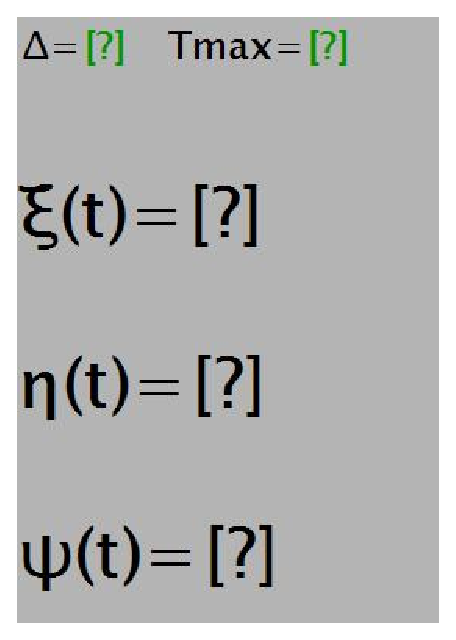
\includegraphics[width=0.5\linewidth]{formul}}
\caption{Система ожидает ввода управления с помощью формул}
\label{ris:formul}
\end{figure}

При наборе формулы поддерживаются следующие действия:
\begin{itemize}
\item{все математические операции (умножение, деление, сложение, вычитание, возведение в степень);}
\item{ввод без ограничения по длине формулы;}
\item{ввод без ограничений по количеству вложенных скобок;}
\item{добавление делегированных тригонометрических и алгебраических функций ($sin(t), cos(t), tg(t), ctg(t), exp(t), ln(t)$ );}
\item{ввод делегированных констант $\pi$ ;}
\item{ввод независимой переменной $t$;}
\end{itemize}

Приоритеты операций в редакторе являются общепринятыми в математике, так, например в выражении $x+y*z$ сначала будет выполнено умножение, а потом сложение. 
	
Кроме того, редактор дает возможность менять приоритеты по умолчанию, указывая их в явном виде с помощью символов парных скобок. При этом глубина вложенности прямо пропорциональна величине приоритета, то есть более внутренние скобки указывают на больший приоритет, чем внешние, обрамляющие их. В предыдущем примере с суммой и произведением порядок вычисления можно поменять, используя скобки, записав всё выражение так:  

\begin{center}
$(x+y)*t$
\end{center}

Очередность ввода компонент уравнения осуществляется путем движения извне вовнутрь. 
Пример  $sin(t)+2*t$, порядок действий ввода:
\begin{enumerate}
\item{Добавить действие сложение;}
\item{Левый аргумент блока сложения заменить на функцию $sin([?])$;}
\item{Добавить переменную времени аргументом функции;}
\item{Правый аргумент блока сложения заменить на блок умножения;}
\item{Левый аргумент блока умножения заменить на число(выделен зеленым);}
\item{Ввести число;}
\item{Правый аргумент блока умножения заменить на переменную времени;}
\end{enumerate}
	
Если все действия проделаны правильно, на заднем плане отрисуется график функции рис.\eqref{ris:formulinput}.

\begin{figure}[h]
\center{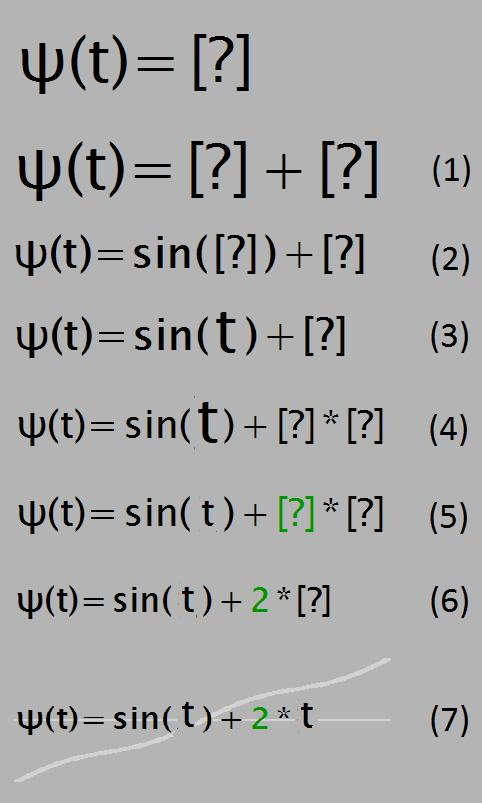
\includegraphics[width=0.5\linewidth]{formulinput}}
\caption{Типичный ввод формулы по этапам функции $sin(t)+2*t$}
\label{ris:formulinput}
\end{figure}

\par
\textbf{Метод ввода траектории движения робота графически}

Если пользователь выбирает графический способ ввода траектории, перед ним открывается поле для поточечного ввода произвольной траектории рис.\eqref{ris:traj}. Изначально поле представляется чистым листом на который можно нанести неограниченное количество точек. Каждая из точек имеет три характеристики (координаты на плоскости и угол поворота). 

Ввод данных организован при помощи двух совокупных плоскостей  $\xi O\psi$, $\eta O\psi$, переключение между которыми производится нажатием на перекрестие в левом нижнем углу. Скорость движения робота в этом случае принимается постоянной на каждом отрезке  ломанной.

При редактировании траектории мгновенно происходит расчет управления и управляемого движения и отображается результат математического моделирования.

\begin{figure}[h]
\center{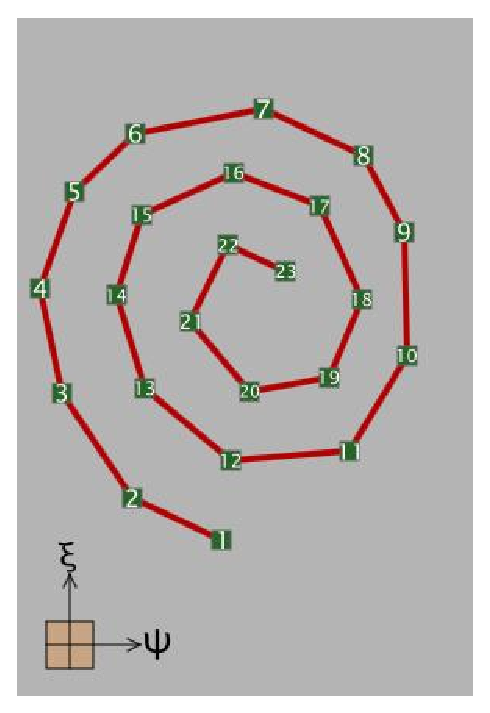
\includegraphics[width=0.5\linewidth]{traj}}
\caption{Внешний вид модуля ввода траектории}
\label{ris:traj}
\end{figure}

Редактор является авторской разработкой и предоставляет возможность поточечного ввода траектории. Модуль позволяет вводить любые значения от -1.7е+308 до 1.7е+308 с точность до 1e-12.
	
Для более подробного ознакомления с модулем ввода траектории см. Приложение 3.

Основные инструменты редактора:
\begin{itemize}
\item{удалить траекторию;}
\item{добавление точки по клику в любой части рабочей области;}
\item{вставить точку в произвольную часть ломаной;}
\item{переместить точку без разрыва траектории;}
\item{удалить узловую точку без разрыва траектории;}
\item{замкнуть траекторию путем соединения }
\end{itemize}

Благодаря векторной графике, лежащей в основе проектирования приложения, в данном модуле поддерживается масштабирование ломаной в широких пределах, что  позволяет пользователю редактировать степень излома траектории. В случае, если траектория скрывается из рабочей области, на границах плоскости появляются ключевые точки, предоставляющие информацию о положении ломаной за пределами рабочей области.
\par
\textbf{Метод ввода файлом массивом данных}

При выборе этого метода ввода, пользователю необходимо загрузить в программу файл с уже сформированным управлением. Данный программный продукт позволяет провести импорт из Microsoft Excell рис.\eqref{ris:mass}. На данный момент программный продукт поддерживает два расширения файла: 

\begin{itemize}
\item{cvs;}
\item{msr - внутреннее расширение.}
\end{itemize}

\begin{figure}[h]
\center{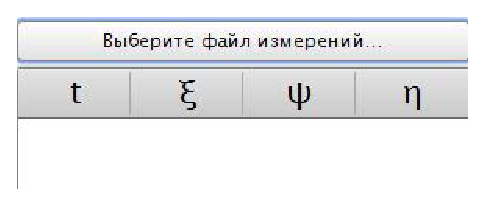
\includegraphics[width=0.5\linewidth]{mass}}
\caption{Внешний вид формы для ввода массива данных}
\label{ris:mass}
\end{figure}

Данные полученные из массива итерационно подставляются в формулы. Данные следуют потоком в следующем порядке:
\begin{itemize}
\item{момент времени  $t_i$;}
\item{значение  $\xi(t_i)$;}
\item{значение  $\psi(t_i)$;}
\item{значение  $\eta(t_i)$;}
\item{символ перехода на новую строку + символ сдвига каретки;}
\end{itemize}

В качества разделителя данных используется символ ";". Дробные числа записываются через символ ",".
Пример:   0,1;4;5;6;.
\par
\textbf{Расчетная часть}

Для детального ознакомления с реализацией расчета см. Приложение 1.
После задания траектории движения робота одним из описанных способов, в правой части приложения выводятся следующие графики рис.\eqref{ris:graph}

\begin{enumerate}
\item{ графики  $\xi(t), \xi_0(t)$ траектории центра масс платформы }
\item{ графики  $\eta(t), \eta_0(t)$ координаты  центра масс платформы }
\item{ графики  $\psi(t), \psi_0(t)$ угла поворота платформы  }
\item{ графики  $\dot{\xi(t)}, \dot{\xi_0(t)}$ скорости центра масс платформы }
\item{ графики  $\dot{\eta(t)}, \dot{\eta_0(t)}$ скорости координаты  центра масс платформы }
\item{ графики  $\dot{\psi(t)}, \dot{\psi_0(t)}$ скорости поворота платформы  }
\item{ графики траектории платформы  на фазовой плоскости $\xi(\eta(t)), \xi_0(\eta_0(t))$}
\item{ графики  $\|\dot{\xi(t)} - \dot{\xi_0(t)}\|$, $\|\dot{\eta(t)} - \dot{\eta_0(t})\|$, 
$\|\dot{\psi(t)} - \dot{\psi_0(t)}\|$  }
\end{enumerate}
При построении графиков  использовался пятиточечный метод численного дифференцирования.

По графикам можно судить, что рассматриваемая система двигается вдоль отслеживаемой траектории на расстоянии, не превышающем погрешности слежения.

\begin{figure}[h]
\center{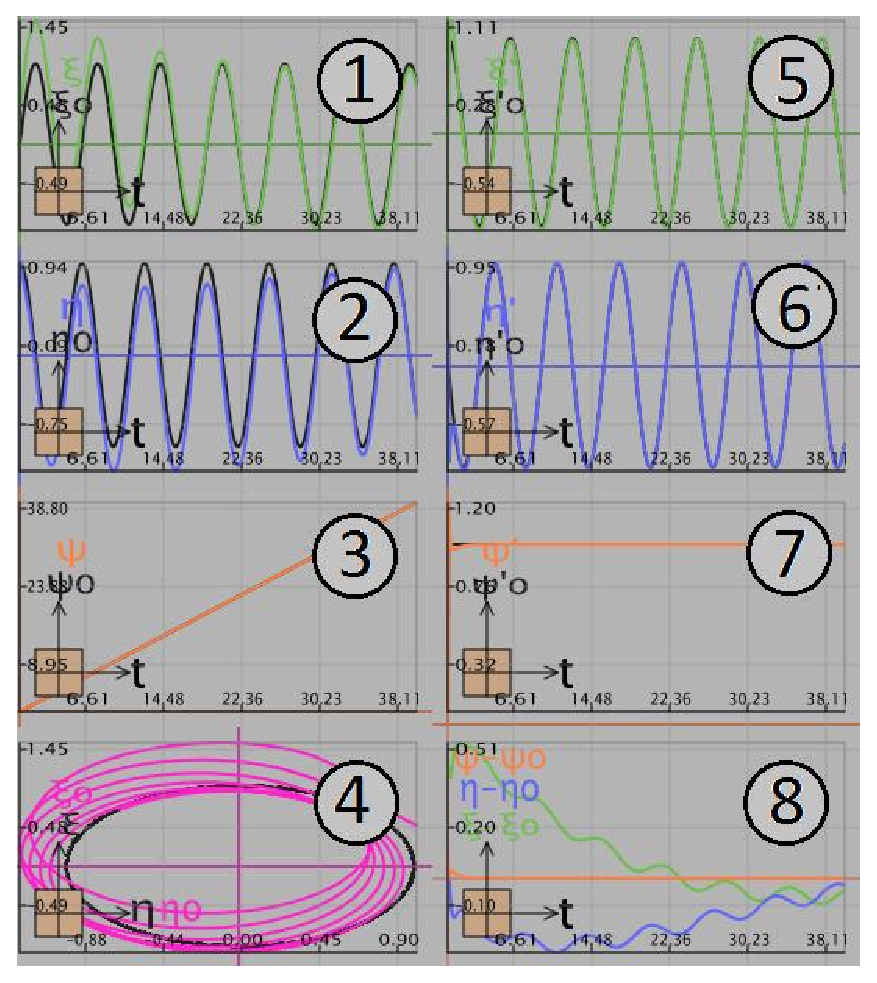
\includegraphics[width=1\linewidth]{graph}}
\caption{Внешний вид расчетной части}
\label{ris:graph}
\end{figure}


